\chapter{Mitigations}
\label{ch:mitigations}
In this chapter we describe the mitigations to the threats we found in
the previous chapter.

\section{Mitigation by Threat}

\section{Risk and Prioritization}
\label{sec:risk}
While it is beyond the scope of this assignment to describe any technical or business processes used to manage risk, we implicitly manage risk through our assumptions and mitigations.  For example, the risk from the threat of loss of the USB (resulting in a denial of service) is transferred to the owner of the device by assuming that the owner will take adequate precautions to prevent loss or theft of the device.  For the unlikely lucky guess threat, the risk is accepted because the likelihood of properly guessing a complex password in a very small, fixed number of tries is unlikely.

\begin{marginfigure}
    \centering
    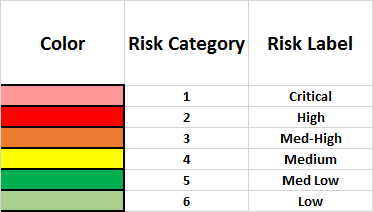
\includegraphics[width=\linewidth]{riskcats}
    \caption{Risk Categories Used in Threat Modeling}
    \label{fig:riskcats}
\end{marginfigure}

In general, we would expect to pay most attention to priority risks in increasing order; for example, a category one risk would be addressed before a category 3 threat risk.

\subsection{Risk Determination}
We used a modified OWASP risk methodology to determine the risks posed by each threat or group of similar threats. Detailed information concerning the assessed risks can be found in appendix 4.;

